\section*{Lente delgada}

\item 
\begin{enumerate}
	\item A partir de la ecuación de la dioptra, considerando dos dioptras esféricas tal que la separación entre ellas sea mucho menor que las restantes longitudes involucradas, deduzca la ecuación para las lentes delgadas.
	\item Analice de qué depende la convergencia o divergencia de una lente.
	\item Grafique la posición de la imagen $s'$ vs. la del objeto $s$ para lentes convergentes y divergentes.
	Analice el aumento en función de $s$, en particular cuando está en el foco \(s = f\) y cuando \(s \rightarrow - \infty\).
	\item ¿Pueden ser iguales (en módulo) los focos de una lente?
	\item Demuestre que la menor distancia objeto--imagen es $4f$, si la lente está inmersa en un único medio.
	\item Dibuje los frentes de onda incidente, refractado por la primer dioptra y refractado por la segunda.
\end{enumerate}



\item Determine la distancia focal \(f\) de una lente plano--cóncava (\(n = \num{1.5}\)) cuyo radio de curvatura es \SI{10}{\centi\metre}.
Determine su potencia en dioptrías que se define como \(D = \frac{1}{f}\) si \(f\) está expresada en \si{\metre}.
Calcule el aumento \(M\) expresado popularmente en unidades de X (e.g. 4X), como \(M = \SI{0.25}{\metre} D + 1\).


\item Se tiene una lente biconvexa con \(R_1 = R_2 = \SI{10}{\centi\metre}\), construida con un vidrio de índice \num{1.5}.
Se la usa con aire a un lado de la misma y con un líquido de índice \num{1.7} al otro lado.
¿Cuánto valen las distancias focales?
¿Es convergente o divergente?
Responda las mismas preguntas si:
\begin{enumerate}
	\item está inmersa sólo en aire,
	\item está inmersa en el medio de índice \num{1.7}.
\end{enumerate}



\item El ancho de la Luna cubre \ang{;31;08} del campo visual humano promedio.
¿Cuál es el tamaño de la imagen de la luna, a través de una lente convergente de distancia focal \SI{1}{\metre}?



\item
\begin{enumerate}
	\item Se coloca un objeto a \SI{18}{\centi\metre} de una pantalla, ¿en qué puntos entre la pantalla y el objeto se puede colocar una lente delgada convergente de distancia focal \SI{4}{\centi\metre}, para que la imagen del objeto esté sobre la pantalla? ¿Qué diferencia hay entre ubicarla en una u otra posición?
	\item Un objeto se halla a distancia fija de la pantalla. Una lente delgada convergente, de distancia focal \SI{16}{\centi\metre}, produce imagen nítida sobre la pantalla cuando se encuentra en dos posiciones que distan entre sí \SI{60}{\centi\metre}.
¿Cuál es la distancia objeto--pantalla?
\end{enumerate}



\item Halle la distancia focal de una lente sumergida en agua, sabiendo que su distancia focal en el aire es de \SI{20}{\centi\metre}.
El índice de refracción del vidrio de la lente es \num{1.6}. 



\item
\begin{minipage}[t][2cm]{0.65\textwidth}
Se tiene una lente delgada en las condiciones que presenta la figura.
Indique en qué punto del eje óptico debe incidir un rayo para que atraviese la lente sin desviarse.
Exprese el resultado en función de la distancia focal objeto y de los índices de refracción.
\end{minipage}
\begin{minipage}[c][0.4cm][t]{0.3\textwidth}
	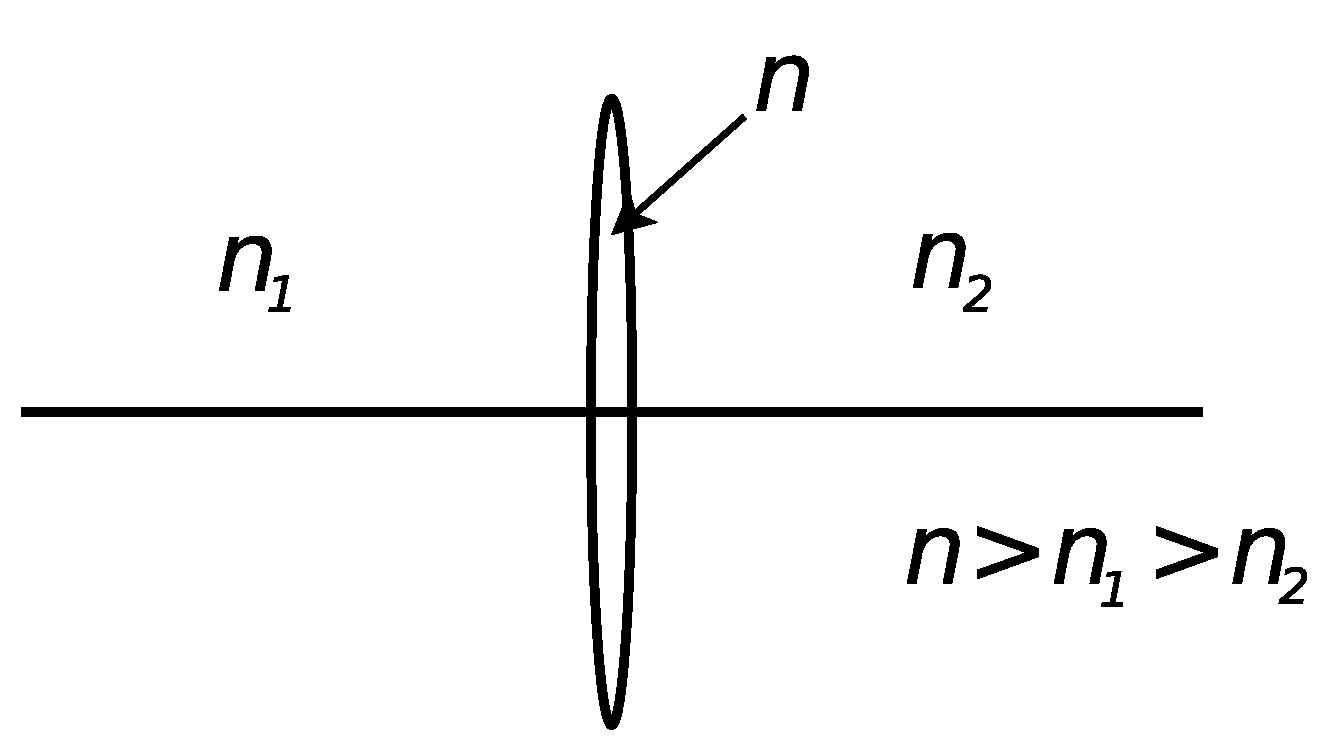
\includegraphics[width=\textwidth]{ej3-25}
\end{minipage}


\item (*) Demostrar que:
\begin{enumerate}
	\item Si un sistema óptico forma imágenes geométricamente perfectas, todos los rayos que conectan puntos conjugados recorren el mismo camino óptico.
	Utilice el principio de Fermat.
	\item Si una lente delgada forma imágenes perfectas sólo en la aproximación paraxial, la diferencia de caminos ópticos entre dos rayos cualesquiera que conectan puntos conjugados y que en todo punto disten menos que $y$, es de orden superior a $y^2$.
\end{enumerate}


\item
\begin{enumerate}
	\item Determine el radio de curvatura de una lupa equiconvexa (\(n = \num{1.5}\)) para que su aumento sea 10X, es decir que al ojo aparenta ser \num{10} veces mayor que su tamaño real.
	¿Dónde se encuentra la imagen, y el objeto?
	\item Calcule el aumento de esta lupa cuando la imagen se encuentra a la distancia de visión clara (\SI{20}{\centi\metre}).
	Discuta las ventajas y desventajas de esta opción.
\end{enumerate}
